\documentclass[12pt]{article}
\usepackage{amsmath}
\usepackage{amsthm}
\usepackage{amssymb}
\usepackage{euscript}
\usepackage{mathrsfs}
\usepackage{bm}
\usepackage{enumitem}
\usepackage{tikz}
\usepackage{mathtools}
\usepackage{float}
\usepackage{hyperref}
\usepackage{boldline}
\usepackage{indentfirst}
\usepackage{environ}
\usetikzlibrary{positioning}

\hypersetup{
    colorlinks=true,
    linkcolor=[RGB]{0,0,128},
    filecolor=magenta,
    urlcolor=cyan,
    citecolor = [RGB]{128,0,128}
}

\newcommand{\makeBox}[2] {
  \newsavebox{#1}
  \begin{lrbox}{#1}{#2}\end{lrbox}
}

\tikzstyle{tableau} = [y = -1cm, every node/.style={transform shape}]

\definecolor{gridColor}{RGB}{19,83,150}
\tikzstyle{dominoStyle} = [color=black, fill=white, rounded corners = .1cm, thick]
\tikzstyle{gridLine} = [color=gridColor, thick]
\tikzstyle{dominoText} = [font=\Large, midway]
\tikzstyle{cycleLine} = [color=green, thick, >->]
\tikzstyle{closedCycleLine} = [color=green, thick]
% \tikzstyle{fixedSquareStyle} = [pattern = crosshatch doats, pattern color=gridColor,  opacity=0.2]
\tikzstyle{fixedSquareStyle} = [color=gridColor,  opacity=0.07]
\tikzstyle{tileText} = [font=\large, midway]

\newcommand{\eps}{.06}
\newcommand{\teps}{\eps * 2}

% first entry is row, starting with 1, second entry is column, third is content
\newcommand{\filledSquare}[3]{\filldraw [dominoStyle] (#2 - 1 + \eps, #1 - 1 + \eps) rectangle + (1 - \teps, 1 -\teps) node [tileText] {$#3$};}
% The fourth entry shifts vertically
\newcommand{\filledSquareShift}[4]{\filldraw [dominoStyle] (#2 - 1 + #4 + \eps, #1 - 1 + \eps) rectangle + (1 - \teps, 1 -\teps) node [tileText] {$#3$};}

\newcommand{\horizontalDomino}[3]{\filldraw [dominoStyle] (#2 - 1 + \eps, #1 - 1 + \eps) rectangle + (2 - \teps, 1 -\teps) node [dominoText] {$#3$};}
\newcommand{\verticalDomino}[3]{\filldraw [dominoStyle] (#2 - 1 + \eps,  #1 - 1 + \eps) rectangle + (1 - \teps,2 -\teps) node [dominoText] {$#3$};}

\newcommand{\horizontalDominoShift}[4]{\filldraw [dominoStyle] (#2 - 1 + #4 + \eps, #1 - 1 + \eps) rectangle + (2 - \teps, 1 -\teps) node [dominoText] {$#3$};}
\newcommand{\verticalDominoShift}[4]{\filldraw [dominoStyle] (#2 - 1 + #4 + \eps,  #1 - 1 + \eps) rectangle + (1 - \teps,2 -\teps) node [dominoText] {$#3$};}

\newcommand{\zeroSquare}[2]{\filldraw [dominoStyle] (#2 - 1 + \eps, #1 - 1 + \eps) rectangle + (1 - \teps, 1 -\teps) node [dominoText] {$0$};}
\newcommand{\zeroSquareShift}[3]{\filldraw [dominoStyle] (#2 - 1 + #3 + \eps, #1 - 1 + \eps) rectangle + (1 - \teps, 1 -\teps) node [dominoText] {$0$};}


\newcommand{\emptyBox}[2]{\filldraw [dominoStyle] (#2 - 1 + \eps, #1 - 1 + \eps) rectangle + (2 - \teps, 2 -\teps);}
\newcommand{\signedBox}[3]{
\filldraw [opacity=0] (#2 - 1 + 1, #1 - 1) rectangle + (1, 2) node [dominoText,opacity=1] {$#3$};
\filldraw [dominoStyle, fill opacity = 0] (#2 - 1 + \eps, #1 - 1 + \eps) rectangle + (2 - \teps, 2 -\teps);
}

\newcommand{\emptyBoxShift}[3]{\filldraw [dominoStyle] (#2 - 1 + #3 + \eps, #1 - 1 + \eps) rectangle + (2 - \teps, 2 -\teps);}
\newcommand{\signedBoxShift}[4]{
\filldraw [opacity=0] (#2 - 1 + 1 + #4, #1 - 1) rectangle + (1, 2) node [dominoText,opacity=1] {$#3$};
\filldraw [dominoStyle, fill opacity = 0] (#2 - 1 + #4 + \eps, #1 - 1 + \eps) rectangle + (2 - \teps, 2 -\teps);
}

% These rows and columns are zero-based
\newcommand{\horizontalGridLine}[3]{\draw [gridLine] (#1, #2) -- + (#3,0);}
\newcommand{\verticalGridLine}[2]{\draw [gridLine] (#1, 0) -- + (0,#2);}
\newcommand{\fixedSquare}[2]{\filldraw [fixedSquareStyle] (#1,#2) rectangle +(1,1);}

% This will have #1 * 2 rows and #2 *2 columns
\newcommand{\gridLines}[2] {
  \pgfmathsetmacro{\verticalEnd}{2 * #1}
  \pgfmathsetmacro{\horizontalEnd}{2 * #2}
  \foreach \vertical in {0,...,#2} {
    \pgfmathsetmacro{\var} {2 * \vertical}
    \verticalGridLine{\var}{\verticalEnd}
  }
  \foreach \horizontal in {0,...,#1} {
    \pgfmathsetmacro{\var} {2 * \horizontal}
    \horizontalGridLine{0}{\var}{\horizontalEnd}
  }
}

% This will have #1 * 2 rows and #2 *2 columns
% The vertical lines will be shifted over #3 squares
\newcommand{\gridLinesShift}[3] {
  \pgfmathsetmacro{\verticalEnd}{2 * #1}
  \pgfmathsetmacro{\horizontalEnd}{2 * #2}
  \foreach \vertical in {0,...,#2} {
    \pgfmathsetmacro{\var} {2 * \vertical + #3}
    \verticalGridLine{\var}{\verticalEnd}
  }
  \foreach \horizontal in {0,...,#1} {
    \pgfmathsetmacro{\var} {2 * \horizontal}
    \horizontalGridLine{#3}{\var}{\horizontalEnd}
  }
}

\newcommand{\fixedSquaresStart}[4]{
  \foreach \row in {#1,...,#2} {
    \foreach \column in {#3,...,#4} {
      \pgfmathsetmacro{\var}{\row + \column}
      \ifodd \var
      \else
        \fixedSquare\column\row
      \fi
    }
  }
}

\newcommand{\fixedSquares}[2]{
  \foreach \row in {0,...,#1} {
    \foreach \column in {0,...,#2} {
      \pgfmathsetmacro{\var}{\row + \column}
      \ifodd \var
        \fixedSquare\column\row
      \fi
    }
  }
}

% This has #1 * 2 rows and #2 * 2 columns
\newcommand{\fixedSquaresForGrid}[2] {
  \pgfmathsetmacro{\rowParameter}{#1 * 2 - 1}
  \pgfmathsetmacro{\columnParameter}{#2 * 2 - 1}
  \fixedSquares{\rowParameter}{\columnParameter}
}

% This has #1 * 2 rows and #2 * 2 columns
% The vertical lines will be shifted over #3 squares
\newcommand{\fixedSquaresForGridShift}[3] {
  \pgfmathsetmacro{\rowParameter}{#1 * 2 - 1}
  \pgfmathsetmacro{\columnStart}{#3}
  \pgfmathsetmacro{\columnEnd}{#2 * 2 - 1 + #3}
  \fixedSquaresStart{0}{\rowParameter}{\columnStart}{\columnEnd}
}


% This will have #1 rows and #2 columns
\newcommand{\typeAGridLines}[2] {
  \foreach \vertical in {0,...,#2} {
    \verticalGridLine{\vertical}{#1}
  }
  \foreach \horizontal in {0,...,#1} {
    \horizontalGridLine{0}{\horizontal}{#2}
  }
}

% This will have #1 rows and #2 columns
% The vertical lines will be shifted over #3 squares
\newcommand{\typeAGridLinesShift}[3] {
  \foreach \vertical in {0,...,#2} {
    \pgfmathsetmacro{\var} {\vertical + #3}
    \verticalGridLine{\var}{#1}
  }
  \foreach \horizontal in {0,...,#1} {
    \horizontalGridLine{#3}{\horizontal}{#2}
  }
}

\newcommand{\Sf}{S_f}
\newcommand{\Sb}{S_b}
\newcommand{\sij}{{S_{ij}}}
\renewcommand{\ss}[2]{{S_{#1,#2}}}

\begin{document}
  For simplicity, I'll talk about $SO(p,q)$ with $p + q$ even.
  This is the basic algorithm.

  The first step is to understand the relationship between a number tableau and its sign tableau.
  In previous algorithms, you could pair a number tableau with any sign tableau of the same shape.
  That's not true any longer.
  To understand the the relationship between a number tableau and its sign tableau, you need first what I've been calling the cycle structure of a domino tableau with grid.
  Cycle structure just involves the open cycles of the tableau, and is just the set of pairs $(\Sb(c), \Sf(c))$ (that is, back square, forward square) for $c$ an open cycle.
  So, for example, these two tableaux have the same cycle structure, namely $\{(\ss23, \ss14), (\ss41, \ss32)\}$.

  \makeBox{\tableauOne}{
      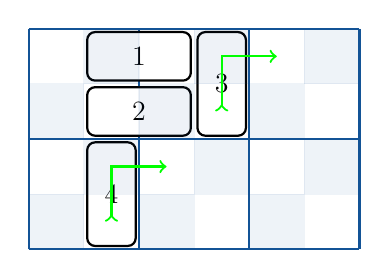
\begin{tikzpicture}[tableau, scale = .7]
        \gridLines{2}{3}
        \horizontalDomino{1}{2}{1}
        \horizontalDomino{2}{2}{2}
        \verticalDomino{1}{4}{3}
        \verticalDomino{3}{2}{4}
        \fixedSquaresForGrid{2}{3}

        \draw[cycleLine] (1.5,3.5) -- ++ (0, -1) -- + (1,0);
        \draw[cycleLine] (3.5, 1.5) -- ++ (0, -1) -- + (1,0);
      \end{tikzpicture}
    }

    \makeBox{\tableauTwo}{
      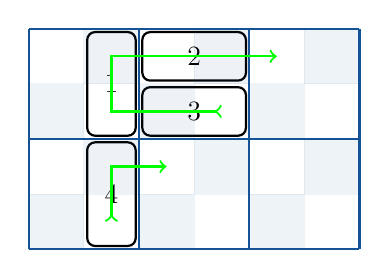
\begin{tikzpicture}[tableau, scale = .7]
        \gridLines{2}{3}
        \verticalDomino{1}{2}{1}
        \horizontalDomino{1}{3}{2}
        \horizontalDomino{2}{3}{3}
        \verticalDomino{3}{2}{4}
        \fixedSquaresForGrid{2}{3}

        \draw[cycleLine] (3.5, 1.5) -- ++ (-2, 0) -- ++ (0, -1) -- + (3, 0);
        \draw[cycleLine] (1.5, 3.5) -- ++ (0, -1) -- + (1, 0);
      \end{tikzpicture}
    }

  \begin{figure}[H]
    \centering
    \begin{tikzpicture}
      \node (C1) {\usebox{\tableauOne}};
      \node[right = of C1] (C2) {\usebox{\tableauTwo}};
    \end{tikzpicture}
  \end{figure}

  The next tableau, on the other hand, has cycle structure $\{(\ss23, \ss32), (\ss41, \ss14)\}$
  In this tableau, the cycle $\{4\}$ is nested in the cycle $\{1, 2, 3\}$.
  For nested cycles, see Definition 3.3.3 of \cite{garfinkle_1993}.
  We'll be seeing more of them.

  \begin{figure}[H]
    \centering
    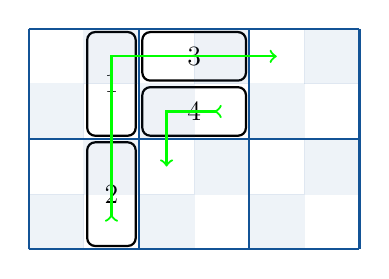
\begin{tikzpicture}[tableau, scale = .7]
      \gridLines{2}{3}
      \verticalDomino{1}{2}{1}
      \verticalDomino{3}{2}{2}
      \horizontalDomino{1}{3}{3}
      \horizontalDomino{2}{3}{4}
      \fixedSquaresForGrid{2}{3}

      \draw[cycleLine] (1.5, 3.5) -- ++ (0, -3) -- + (3, 0);
      \draw[cycleLine] (3.5, 1.5) -- ++ (-1, 0) -- + (0, 1);
    \end{tikzpicture}
  \end{figure}

  In the $SO(p,q)$ algorithm, sign tableaux also have a cycle structure, about which I'll say more in a bit.
  A number tableau and its sign tableau have the same cycle structure.
  Here are some examples.

  \begin{figure}[H]
    \centering
    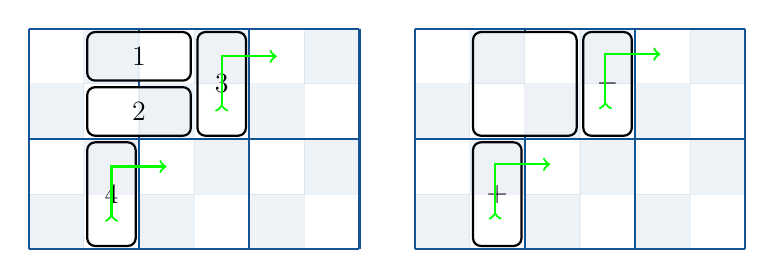
\begin{tikzpicture}[tableau, scale = .7]
      \gridLines{2}{3}
      \horizontalDomino{1}{2}{1}
      \horizontalDomino{2}{2}{2}
      \verticalDomino{1}{4}{3}
      \verticalDomino{3}{2}{4}
      \fixedSquaresForGrid{2}{3}

      \draw[cycleLine] (1.5,3.5) -- ++ (0, -1) -- + (1,0);
      \draw[cycleLine] (3.5, 1.5) -- ++ (0, -1) -- + (1,0);

      \gridLinesShift{2}{3}{7}
      \emptyBoxShift{1}{2}{7}
      \verticalDominoShift{1}{4}{-}{7}
      \verticalDominoShift{3}{2}{+}{7}
      \fixedSquaresForGridShift{2}{3}{7}

      \draw[cycleLine] (1.5 + 7 -.04, 3.5 -.04) -- ++ (0, -1) -- + (1,0);
      \draw[cycleLine] (3.5 + 7 -.04, 1.5 -.04) -- ++ (0, -1) -- + (1,0);
    \end{tikzpicture}
  \end{figure}

  \bigskip

  \begin{figure}[H]
    \centering
    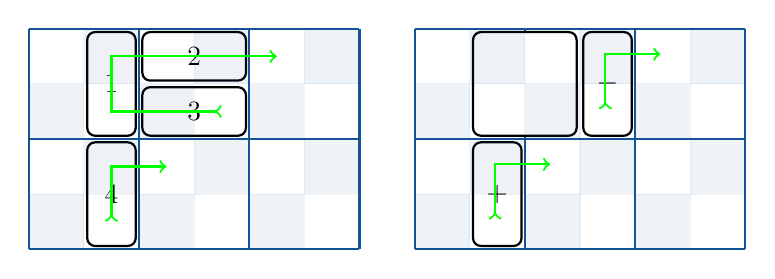
\begin{tikzpicture}[tableau, scale = .7]
      \gridLines{2}{3}
      \verticalDomino{1}{2}{1}
      \horizontalDomino{1}{3}{2}
      \horizontalDomino{2}{3}{3}
      \verticalDomino{3}{2}{4}
      \fixedSquaresForGrid{2}{3}

      \draw[cycleLine] (3.5, 1.5) -- ++ (-2, 0) -- ++ (0, -1) -- + (3, 0);
      \draw[cycleLine] (1.5, 3.5) -- ++ (0, -1) -- + (1, 0);

      \gridLinesShift{2}{3}{7}
      \emptyBoxShift{1}{2}{7}
      \verticalDominoShift{1}{4}{-}{7}
      \verticalDominoShift{3}{2}{+}{7}
      \fixedSquaresForGridShift{2}{3}{7}

      \draw[cycleLine] (1.5 + 7 -.04, 3.5 -.04) -- ++ (0, -1) -- + (1,0);
      \draw[cycleLine] (3.5 + 7 -.04, 1.5 -.04) -- ++ (0, -1) -- + (1,0);
    \end{tikzpicture}
  \end{figure}

  \bigskip

  \begin{figure}[H]
    \centering
    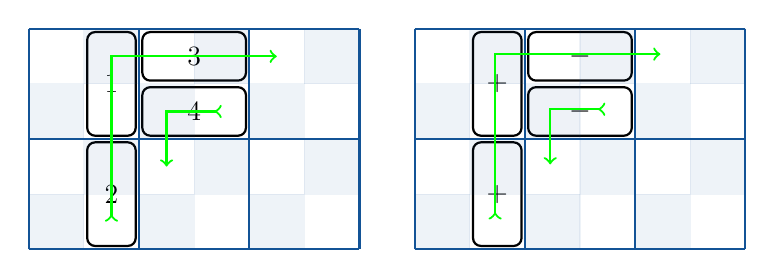
\begin{tikzpicture}[tableau, scale = .7]
      \gridLines{2}{3}
      \verticalDomino{1}{2}{1}
      \verticalDomino{3}{2}{2}
      \horizontalDomino{1}{3}{3}
      \horizontalDomino{2}{3}{4}
      \fixedSquaresForGrid{2}{3}

      \draw[cycleLine] (1.5, 3.5) -- ++ (0, -3) -- + (3, 0);
      \draw[cycleLine] (3.5, 1.5) -- ++ (-1, 0) -- + (0, 1);

      \gridLinesShift{2}{3}{7}
      \verticalDominoShift{1}{2}{+}{7}
      \verticalDominoShift{3}{2}{+}{7}
      \horizontalDominoShift{1}{3}{-}{7}
      \horizontalDominoShift{2}{3}{-}{7}
      \fixedSquaresForGridShift{2}{3}{7}

      \draw[cycleLine] (1.5 + 7 -.04, 3.5 -.04) -- ++ (0, -3) -- + (3, 0);
      \draw[cycleLine] (3.5 + 7 -.04, 1.5 -.04) -- ++ (-1, 0) -- + (0, 1);
    \end{tikzpicture}
  \end{figure}

  The cycles in a sign tableau are a ``minimal representation'' of the cycle structure of the number tableau.
  Minimal here means that they take the minimal number of dominos, but also that they are as far down and to the right as possible.
  The rest of the space is filled with empty 2x2 boxes.
  For example:

  \begin{figure}[H]
    \centering
    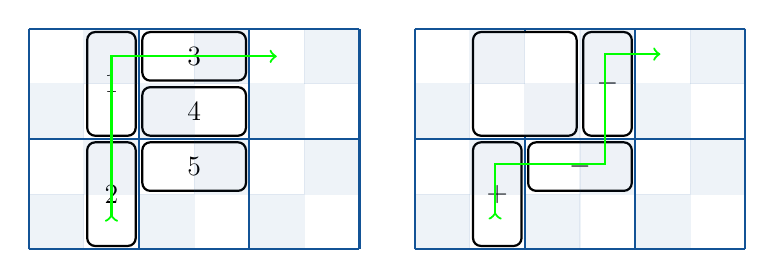
\begin{tikzpicture}[tableau, scale = .7]
      \gridLines{2}{3}
      \verticalDomino{1}{2}{1}
      \verticalDomino{3}{2}{2}
      \horizontalDomino{1}{3}{3}
      \horizontalDomino{2}{3}{4}
      \horizontalDomino{3}{3}{5}
      \fixedSquaresForGrid{2}{3}

      \draw[cycleLine] (1.5, 3.5) -- ++ (0, -3) -- + (3, 0);

      \gridLinesShift{2}{3}{7}
      \emptyBoxShift{1}{2}{7}
      \verticalDominoShift{1}{4}{-}{7}
      \verticalDominoShift{3}{2}{+}{7}
      \horizontalDominoShift{3}{3}{-}{7}
      \fixedSquaresForGridShift{2}{3}{7}

      \draw[cycleLine] (1.5 + 7 -.04, 3.5 -.04) -- ++ (0, -1) -- ++ (2, 0) -- ++(0, -2) -- ++(1, 0);
    \end{tikzpicture}
  \end{figure}
  In the example, both cycles have the minimal number of dominoes, but only the one on the right is also minimal in being pushed down and to the right.

  It might be hard at first to envision cycles without numbers in the dominoes.
  However, their being minimal in this sense gives you a way to do that.
  You start with the most nested cycles and place their dominos, along the bottom right edges of the tableau shape.
  Then the next most nested cycles, and so on.

  Now I have to talk a little more about cycles.
  Cycles can be either boxed or unboxed, that is, all the dominos in the cycle are either boxed or unboxed.
  Also, cycles can be up cycles or down cycles.
  See Definition 3.3.9 of \cite{garfinkle_1993}.
  Actually, in hindsight, this terminology may be confusing.
  An open up cycle is one which moves up, that is, its back square is lower than its forward square.
  If it moves up, one might think that it starts out down.
  So maybe I should have reversed the names.
  But, it's too late now to change it.

  So, there are four types of cycles, up and boxed, up and unboxed, down and boxed, and down and unboxed.
  If you move through a cycle which is up and boxed, it becomes down and unboxed, etc.
  So, we can group cycles into two types, Type I and Type II, let's say, so that a cycle remains the same type when it is moved through.
  Type I cycles are either up and boxed, or down and unboxed.
  Type II cycles are either down and boxed, or up and unboxed.

  Now let's return to the idea of nested open cycles.
  Recall that we are in type $D$.
  When thinking about nested cycles, we can group open cycles into levels.
  Level 1 are cycles which are not nested.
  Level 2 cycles are nested in level 1 cycles.
  And so on.
  Now (again, this is just type $D$), it happens that if the cycle is in an odd level, it is type I, that is, either up and boxed, or down and unboxed.
  If it is in an even level, it is type II.

  With this terminology, I can say more about the tableaux in the algorithm.
  The number tableaux that arise in the algorithm need not be special, but they are not arbitrary.
  Specifically, any open Type I cycle has to boxed.
  Open Type II cycles can be boxed or unboxed.
  (Of course, once the algorithm is done, you can move through all the open unboxed cycles to get the special tableau which is your goal.)

  The relation between the two number tableaux is as follows.
  Starting with one of them, you take the transpose.
  (Recall, transpose is like with a matrix.)
  Now, the $D$ grid is not preserved by transpose.
  If you take a $D$ tableau and transpose it and then put it back on a $D$ grid, all the cycles which were originally boxed are now unboxed, and vice versa.
  However, since also up cycles have become down cycles by tranposing, type I cycles stay type I, and type II cycles stay type II.
  To go from one number tableau in the algorithm to the other, you transpose it and then move through all the Type I cycles.

  Now let me talk more about the sign tableaux.
  A sign tableau, as we've seen, is made up of 2x2 boxes, with no signs in them, and dominos, which may or may not have signs in them.
  More specifically, for every domino in a sign tableau, there is a corresponding domino in the other sign tableau.
  If a domino in a sign tableau has fixed square $\sij$, then the corresponding domino in the other sign tableau is the one with fixed square $S_{ji}$.
  The rule for corresponding dominos is, if a domino in a sign tableau has a sign in it, then the corresponding domino in the other sign tableau doesn't, and vice versa.

  % \bibliographystyle{halpha}
  % \bibliography{biblio}
\end{document}
